%%%%%%%%%%%%%%%%
% kamera

\section{Pohyb kamery}

Aby bylo intro dynamická, potřebujeme v ní pohyb.
Jedním ze způsobů, jak toho můžeme dosáhnout je pohybovat s kamerou.
Správný pohyb kamery může vytvořit i z nezajímavé scény akční podívanou.
Kamera v průběhu času sleduje jistou trajektorii.
Jelikož má intro omezenou velikost, nemůžeme si uložit pro každý krok času, pozici kamery.
Místo toho, si budeme ukládat jen klíčové body a místa mezi nimi budeme vypočítávat z okolních klíčových bodů.

Jeden klíčový bod si můžeme představit jako deset čísel $K=(p,z,y,a)$.
Vektor $p=(p_x,p_y,p_z)$ reprezentuje pozici kamery.
Vektor $z=(z_x,z_y,z_z)$ reprezentuje pohledový vektor neboli směr, kam je kamera nasměrována.
Vektor $y=(y_x,y_y,y_z)$ je vektor určující směr nahoru.
Tento vektor udává natočení kamery podél osy $z$.
Číslo $a$ udává zorný úhel.
Sekvence klíčových bodů definuje pohyb kamery.

Mezi klíčovými body budeme interpolovat.
Pro interpolaci použijeme Catmull-Rom interpolaci popsanou v \cite{CATMULLROM}.
Pro výpočet interpolace z hodnoty $v_1$ do hodnoty $v_2$ používá metoda také hodnoty $v_0,v_3$.
\begin{equation}
\label{eq:catmull0}
v(t)=[t^0,t^1,t^2,t^3]\cdot
\frac{1}{2}\cdot
\left[
\begin{array}{cccc}
 0 &  2 &  0 &  0 \\
-1 &  0 &  1 &  0 \\
 2 & -5 &  4 & -1 \\
-1 &  3 & -3 &  1
\end{array}
\right]
\cdot
\left[
\begin{array}{c}
v_{0} \\
v_{1} \\
v_{2} \\
v_{3} 
\end{array}
\right]
=
C(t) \cdot 
\left[
\begin{array}{c}
v_{0} \\
v_{1} \\
v_{2} \\
v_{3} 
\end{array}
\right]
\end{equation}
Hodnoty $v_0,v_1,v_2,v_3$ jsou klíčové hodnoty.
Hodnota $v(t)$ je interpolovaná hodnota mezi $v_1,v_2$.
Parametr $t$ může nabývat hodnot $t \in \langle 0,1 \rangle$.
Pokud je parametr $t=0$ je hodnota $v(t)=v_1$.
Pokud je parametr $t=1$ je hodnota $v(t)=v_2$.
Funkce $C: \langle 0,1 \rangle \to \mathbb{R}^4$ vrací vektor vah pro parametr $t$.

Pokud máme více než čtyři klíčové hodnoty, interpolujeme po částech.
Například máme $n$ klíčových hodnot $v_1,v_2,\dotsc,v_n$.
Celková délka je $T_{max}$.
Pokud budeme potřebovat hodnoty $v_{1-a}$ respektive $v_{n+a}$, $a \in \mathbb{N}$, použijeme $v_1$ respektive $v_n$.
Výsledná hodnota v místě $t$ je dána podle vztahu:
\begin{equation}
v(t)=C \left((n-1)\frac{t}{T_{max}}-i\right)\cdot
\left[
\begin{array}{c}
v_{i} \\
v_{i+1} \\
v_{i+2} \\
v_{i+3} 
\end{array}
\right]
\end{equation}
Index $i \in \{0,1,\dotsc,n-2\}$ udává segment, ve kterém se interpoluje z klíčových hodnot.
Jeho hodnota je:
\begin{equation}
i=\left \lfloor \frac{t}{T_{max}} \cdot (n-1) \right \rfloor
\end{equation}
Interpolaci budeme provádět pro všech deset čísel klíčového bodu.
Získáme tak pro čas $t$ přesný popis kamery.

\subsection{Efekty kamery}
Pokud již máme vyřešený pohyb kamery, je vhodné jej dobře použít.
V intru můžeme použít několik efektů, které vidíme například ve filmech.
Prvním z nich je efekt, kdy se kamera přibližuje k objektu a její zorný úhel se zvětšuje.
Situace je znázorněna na obrázku \ref{fig:kamera0}.
Objekt by se důsledkem zmenšení vzdálenosti od kamery měl zvětšovat.
Pokud budeme ale zároveň zvětšovat zorný úhel, zůstane stejně velký.
Okolí kolem objektu se ale bude roztahovat do šíře.
Obdobný efekt lze vytvořit obráceně.
Místo abychom se k objektu přibližovali, budeme se vzdalovat a zorný úhel zmenšovat.
Tento efekt je oblíbený mezi filmaři.
Efekt bývá využíván v chodbách, tunelech a podobných protáhlých prostorách, kde je zvýrazněn.
\begin{figure}[h]
\centering
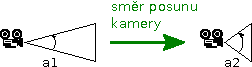
\includegraphics[width=7.5cm,keepaspectratio]{obr/kamera0.pdf}
\caption{Efekt kamery s využitím zorného úhlu.
Kamera se posouvá zleva doprava.
Její zorný úhel se přitom zvětšuje $a_1<a_2$}
\label{fig:kamera0}
\end{figure}

Další efekt je rovněž hojně používaný ve filmech.
Kamera se zaměří na jeden objekt, přiblíží na něj pomocí zmenšení zorného úhlu a rotuje kolem něj.
Efekt je znázorněn obrázkem \ref{fig:kamera1}.
Objekt je snímán na stejném místě.
Vzdálená krajina se ale rychle pohybuje na pozadí.
Bývá používán v exteriérech, kdy význačný objekt stojí na vrcholku hory nebo kopce.
\begin{figure}[h]
\centering
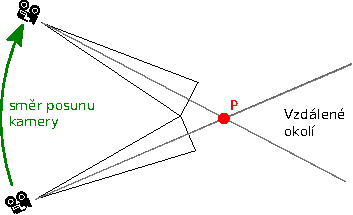
\includegraphics[width=7.5cm,keepaspectratio]{obr/kamera1.pdf}
\caption{Efekt kamera kdy se kamera zaměří na jeden bod $P$ a rotuje kolem něj.}
\label{fig:kamera1}
\end{figure}

